\documentclass[11pt,a4j,uplatex]{jsarticle}
\usepackage{ascmac}
\usepackage{amsmath}
\usepackage[dvipdfmx]{graphicx}
\usepackage{upgreek}

\newsavebox{\circlebox}
\savebox{\circlebox}{\fontencoding{OMS}\selectfont\Large\char13}
\newlength{\circleboxwdht}
\newcommand{\centercircle}[1]{%
  \setlength{\circleboxwdht}{\wd\circlebox}%
  \addtolength{\circleboxwdht}{\dp\circlebox}%
  \raisebox{0.4\dp\circlebox}{%
    \parbox[][\circleboxwdht][c]{\wd\circlebox}{\centering#1}}%
  \llap{\usebox{\circlebox}}%
}	%丸数字(文字)環境。\centercircle{入れたい文字} で丸文字を表示する。


\title{宮島研究室2019年度B4スタート実験}
\author{東京理科大学 応用物理学科 宮島研究室B4 渡辺慧}
\date{\today}


\begin{document}

\maketitle %タイトル

\thispagestyle{empty}%このページにはページ番号を入れない.
\clearpage
\addtocounter{page}{-1}%ページのカウントを-1する.

\newpage

\tableofcontents %目次

\thispagestyle{empty}%このページにはページ番号を入れない
\clearpage
\addtocounter{page}{-1}

%\listoffigures%図目次。確認用。後で消す

\newpage
\section{本研究の目的}
なんとか

\section{原理}
\subsection{X線回折}
\subsection{回折条件}
\subsection{逆格子空間}
\subsection{NaCl粉末の回折パターン}

$2\theta$の値が90よりも小さいときの、NaCl粉末の回折パターンを表\ref{data}に示す。実験データの解析のおいては、この表のデータを参照する。

\begin{table}[htbp]
 \begin{center}
  \caption{NaCl粉末の回折パターン\cite{powder}.}
  \begin{tabular}{|r|r|r|r|r|r|}  \hline
                           & \multicolumn{3}{c|}{} &   &                                \\
   $2\theta(\mathrm{deg})$ & h                     & k & l & Intensity & d-spacing [nm] \\  \hline \hline
   26.886                  & 1                     & 1 & 1 & 10        & 0.3312         \\
   31.145                  & 2                     & 0 & 0 & 99        & 0.2869         \\
   44.629                  & 2                     & 2 & 0 & 61        & 0.2028         \\
   52.878                  & 3                     & 1 & 1 & 3         & 0.173          \\
   55.426                  & 2                     & 2 & 2 & 19        & 0.1656         \\
   64.959                  & 4                     & 0 & 0 & 8         & 0.1434         \\
   71.633                  & 3                     & 3 & 1 & 2         & 0.1316         \\
   73.797                  & 4                     & 2 & 0 & 19        & 0.1283         \\
   82.251                  & 4                     & 2 & 2 & 13        & 0.1171         \\
   88.472                  & 5                     & 1 & 1 & 2         & 0.1104         \\ \hline
  \end{tabular}
  \label{data}
 \end{center}
\end{table}

\newpage
\section{NaCl粉末及び単結晶の回折パターンの観測方法}

NaCl粉末及び単結晶の回折パターンを、X線回折装置"SmartLab"を用いて観測した。$\mathrm{SmartLab}$の構造を図\ref{smartlab}に示す。

\begin{figure}[htb]
 \centering
 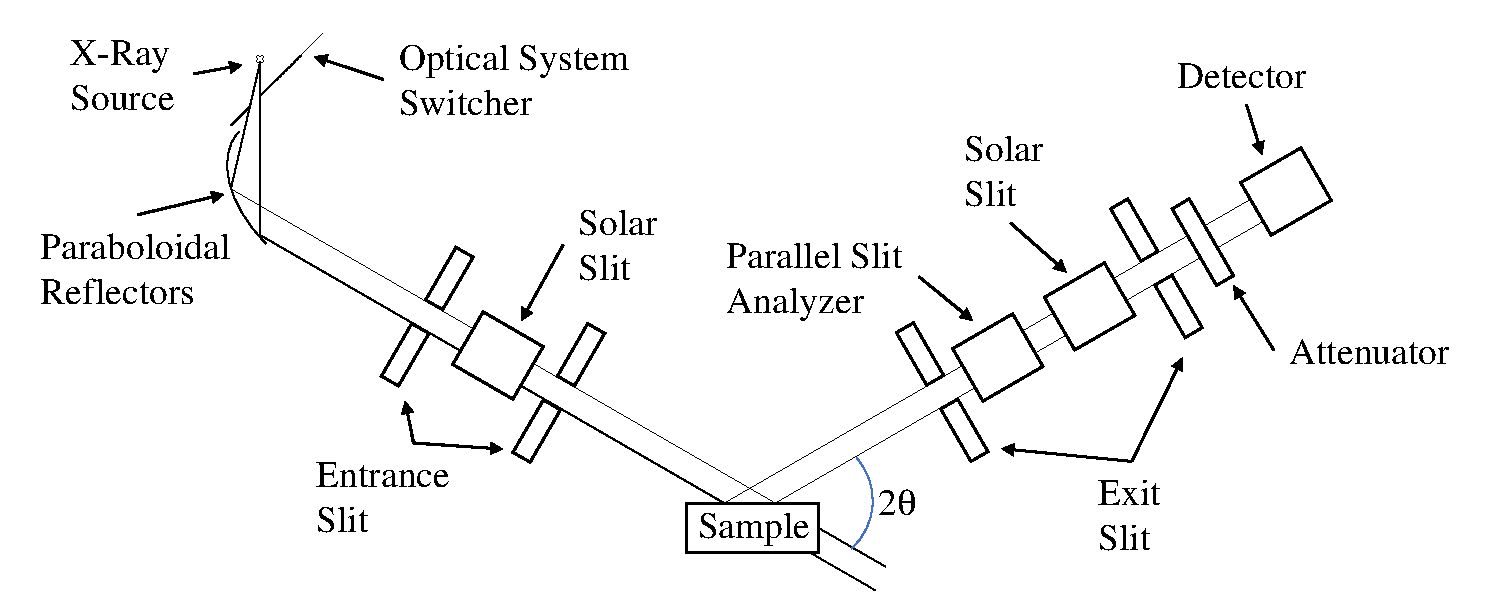
\includegraphics[clip,width=12cm]{XRD.eps}
 \caption{SmartLabの内部構造.}
 \label{smartlab}
\end{figure}

X線源から放射された光をNaCl粉末及び単結晶に照射し、光検出器で回折光を観測した。X線源から等方的に放射された光を、放物面人工多層膜ミラーを用いて単色化・平行化し、2枚の入射スリットとソーラースリットを用いて発散を制限した。2枚の出射スリットとソーラースリットを用いて、試料からの回折光の発散を制限した。アッテネーターを用いて、光検出器に入射する光を減衰させた。PSA(平行スリットアナライザー)を用いて分解能を決定した。$2\theta$は入射光と出射光のなす角である。表\ref{exp}の実験条件の下試料ごとに$2\theta$を変えてゆき、回折パターンを測定した。試料はNaCl粉末とNaCl単結晶の2種類である。NaCl単結晶の寸法を図\ref{size}に示す。

\begin{table}[ht]
 \centering
 \caption{実験条件.}
 \begin{tabular}{lc}\hline
  \multicolumn{2}{c}{実験条件}          \\ \hline
  入射スリット     & 1 mm               \\
  出射スリット     & 1 mm               \\
  ソーラースリット & 0.5 deg            \\
  X線波長          & 1.543\AA、1.392\AA \\\hline
 \end{tabular}
 \label{exp}
\end{table}

\begin{figure}[htb]
 \centering
 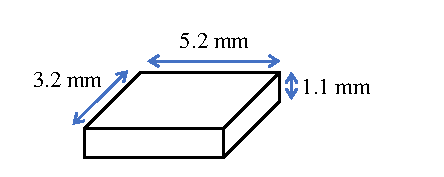
\includegraphics[clip,width=9cm]{bulk.eps}
 \caption{NaCl単結晶の寸法.}
 \label{size}
\end{figure}

\newpage
縦3.2 mm、横5.2 mm、高さ1.1 mmの結晶を、最も面積の広い面を下にして試料台に設置した。

\newpage
\section{NaCl粉末及び単結晶の回折パターンの解析}


\subsection{NaCl粉末}

NaCl粉末における回折パターンを図\ref{powder}に示す。

\begin{figure}[htb]
 \centering
 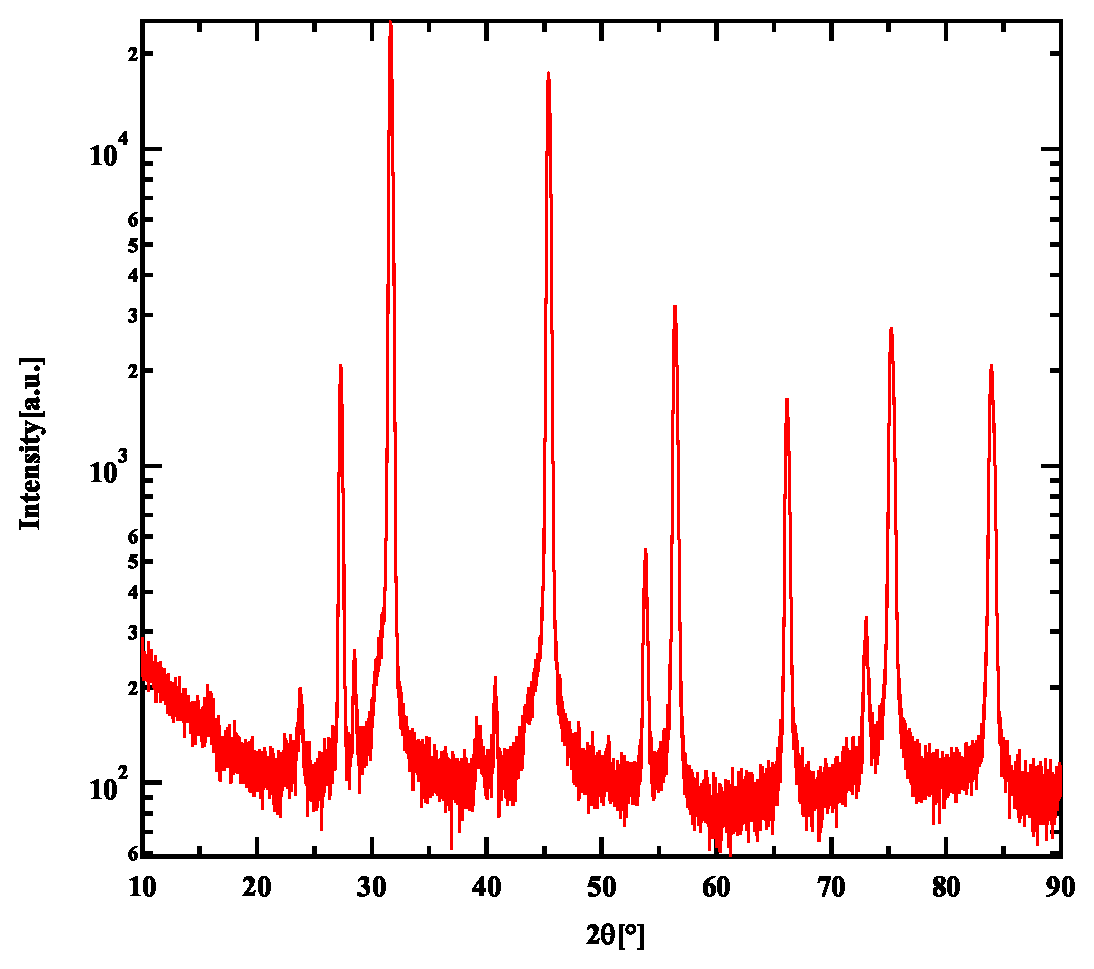
\includegraphics[clip,width=7cm]{FigPowder.eps}
 \caption{NaCl粉末の回折パターン.}
 \label{powder}
\end{figure}

横軸はAの回転角、縦軸は回折強度である。グラフから、鋭いピークが複数見られる。これらのピークのうち、頂点における$2\theta$が、表\ref{data}の値と近いものだけを抜き出したものを表\ref{pow}に示す。

\begin{table}[htbp]
 \begin{center}
  \caption{NaCl粉末の格子定数.}
  \begin{tabular}{|c|r|c|lll|c|}  \hline
   $2\theta[\mathrm{deg}]$ & \multicolumn{1}{c|}{$2\theta[\mathrm{rad}]$} & $G_{m}$     & h & k & l & a           \\ \hline  \hline
   27.306                  & 0.468753                                     & 1.891361571 & 1 & 1 & 1 & 5.751031023 \\
   31.646                  & 0.543256333                                  & 2.185068392 & 2 & 0 & 0 & 5.748103832 \\
   45.397                  & 0.779315167                                  & 3.093719005 & 2 & 2 & 0 & 5.741478885 \\
   53.828                  & 0.924047333                                  & 3.63032518  & 3 & 1 & 1 & 5.737338297 \\
   56.419                  & 0.968526167                                  & 3.791544409 & 2 & 2 & 2 & 5.737650888 \\
   66.178                  & 1.136055667                                  & 4.381295096 & 4 & 0 & 0 & 5.733464524 \\
   73.041                  & 1.2538705                                    & 4.777872498 & 3 & 3 & 1 & 5.729304283 \\
   75.259                  & 1.291946167                                  & 4.902560146 & 4 & 2 & 0 & 5.728642375 \\
   83.979                  & 1.4416395                                    & 5.375122452 & 4 & 2 & 2 & 5.723700519 \\  \hline
  \end{tabular}
  \label{pow}
 \end{center}
\end{table}

\newpage
逆格子ベクトルの大きさ$G_{m}$は
\begin{equation}
 G_m=\frac{4\pi}{\uplambda}\sin\theta
 \label{gyakukousi}
\end{equation}
で計算した。$\uplambda$は、今回は$K_\alpha$線の波長である1.543 nmを用いた。格子定数$a$は、$G_{m}$から
\begin{equation}
 a=\frac{2\pi}{G_m}\sqrt{h^2+k^2+l^2}
 \label{kousiteisuu}
\end{equation}
で計算した。各$\theta$におけるaの平均をとって、格子定数は
\begin{equation}
 a=5.736746
 \label{complete}
\end{equation}
と求まった。

\newpage
\subsection{NaCl単結晶}

図\ref{bulk}に示す。

\begin{figure}[htb]
 \centering
 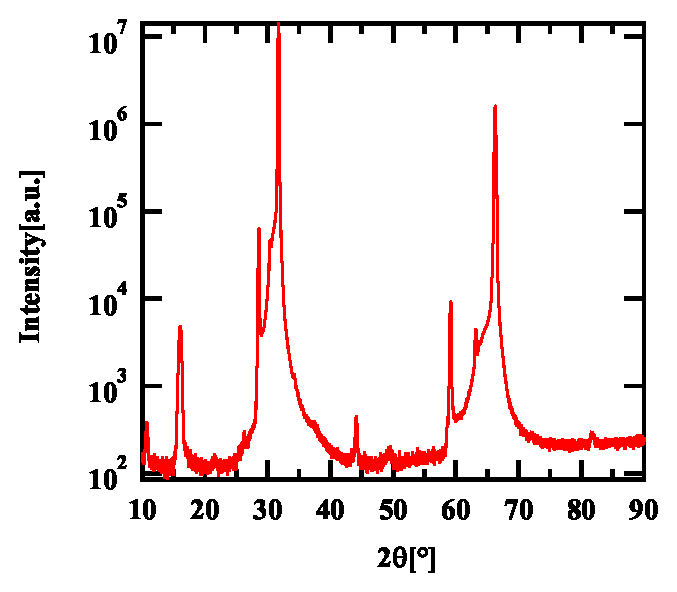
\includegraphics[clip,width=9cm]{FigBulk.eps}
 \caption{NaCl単結晶の回折パターン.}
 \label{bulk}
\end{figure}

横軸はAの回転角、縦軸は回折強度である。グラフから、鋭いピークが複数見られる。$2\theta/\theta$法を用いた単結晶のX線回折測定では、[001]面に平行な面での回折しか観測できない。そこで、(h,k,l)=(0,0,2n)となるように回折指数をとり、粉末試料で得た格子定数に近い計算結果が得られるよう、逆算をして$2\theta$を定めた。その結果を表\ref{crystal}に示す。

\begin{table}[htbp]
 \begin{center}
  \caption{NaCl単結晶の格子定数.}
  \begin{tabular}{|c|c|c|c|ccc|c|c|c|}  \hline
   $2\theta[\mathrm{deg}]$ & $2\theta[\mathrm{rad}]$ & $G_{m\beta}$ & $G_{m\alpha}$ & h & k & l & $a_\beta$   & $a_\alpha$  & $a$         \\   \hline  \hline
   28.598                  & 0.490932333             & 2.195818211  & 1.982945083   & 0 & 0 & 2 & 5.71996349  & 6.334013034 & 5.71996349  \\
   31.739                  & 0.544852833             & 2.431301177  & 2.195599203   & 0 & 0 & 2 & 5.165958095 & 5.72053405  & 5.72053405  \\
   59.173                  & 1.015803167             & 4.394597543  & 3.968564221   & 0 & 0 & 4 & 5.716109326 & 6.329745117 & 5.716109326 \\
   66.28                   & 1.137806667             & 4.867753959  & 4.395850588   & 0 & 0 & 4 & 5.160490899 & 5.714479939 & 5.714479939 \\  \hline
  \end{tabular}
  \label{crystal}
 \end{center}
\end{table}

この逆算から、特性X線$K_\alpha$と$K_\beta$による1次と2次の回折角が得られた。それを図\ref{kakb}に示す。

\begin{figure}[htb]
 \centering
 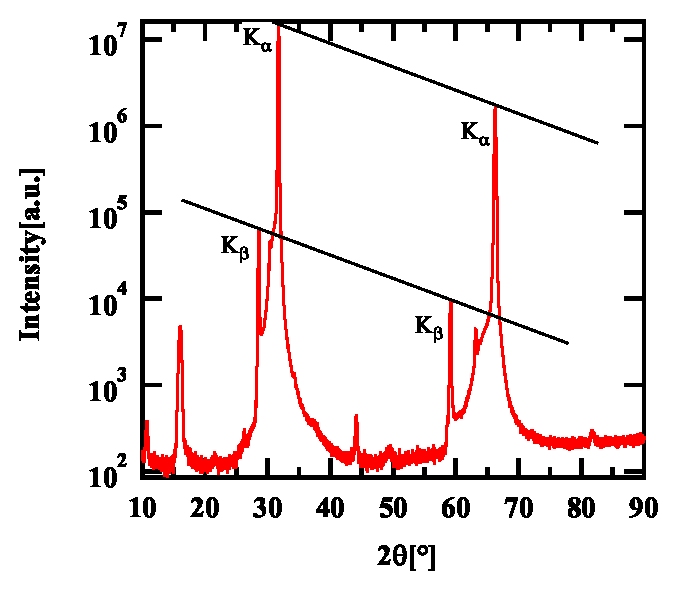
\includegraphics[clip,width=9cm]{kakb.eps}
 \caption{NaCl結晶の回折パターン.}
 \label{kakb}
\end{figure}

\newpage

ブラッグの回折条件より、$2d\sin\theta=n\lambda$である。よって、表\ref{kakb}の値から、[001]方向の面間隔を計算できる。計算結果を表\ref{d}に示す。

\begin{table}[htbp]
 \begin{center}
  \caption{NaCl単結晶の面間隔.}
  \begin{tabular}{|l|l|}  \hline
   2[deg] & d           \\  \hline  \hline
   28.598 & 2.859981745 \\
   31.739 & 2.861717794 \\
   59.173 & 2.858054663 \\
   66.28  & 2.858689203 \\ \hline
  \end{tabular}
  \label{d}
 \end{center}
\end{table}

各$\theta$における$d$の平均をとって、面間隔は
\begin{equation}
 d=2.859610851
 \label{fin}
\end{equation}
と求まった。

\section{結論}
かんとか

\newpage
%参考文献。\cite{タグ}で参照を示せる。
\begin{thebibliography}{9}
 \bibitem{powder}株式会社島津 https://www.shimadzu.co.jp/products/opt/guide/07.html 2019/4/12
 \bibitem{CCD} キヤノンサイエンスラボ https://global.canon/ja/technology/s\_labo/light/003/04.html 2019/04/12
 \bibitem{Fibor} 分光計器株式会社 http://www.bunkoukeiki.co.jp/technology.fiber.html 2019/04/12
 \bibitem{varshni}Y.P.Varshni TEMPERATURE DEPENDENCE OF THE ENERGY GAP IN SEMICONDUCTORS
 \bibitem{gapE}キッテル固体物理学入門上第8版 p.119


\end{thebibliography}

\end{document}
